\chapter{Optimal City Size}

\section{Public good theory and the size of cities}

The theory of public goods is used in urban economics  to produce a surprising result. A simple ``monocentric city'' with a public good at the centre has an optimal size. The result follows from the fact that the a public good has a fixed cost- independent of the population, but transport costs rise for people who live farther from the centre.


With a low population, adding people spreads the fixed cost of the public good over more people and the average cost falls. Eventually the rising cost of transportation causes average cost to rise. Just as in the theory of the firm, there is a minimum average cost, of output, in urban theory we get a minimum average cost of providing a public good, and that gives us the optimal city size. 


The model is actually quite general. In place of public goods we could  have network or or production externalities driving growth. as well as  simple time and fuel costs for individuals we could take into account congestion, pollution, and rising infrastructure costs.



\begin{figure}
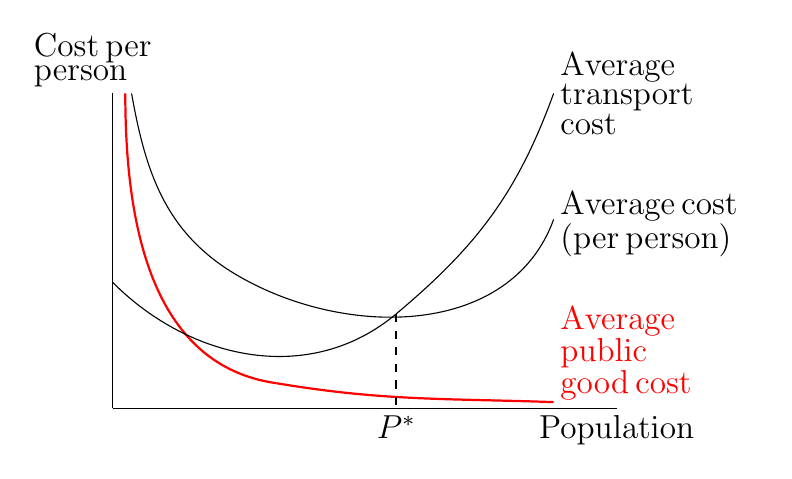
\begin{tikzpicture}[scale=0.8]
\tiny
\draw (0,0) -- (8,0) node [below] {\large Population};
\draw (0, 0) -- (0,5) node [above, text width=2cm] {\large Cost per person};
\draw [red, thick] (0.2,5) to [out=270,in=172] (2.6,0.4);
\draw[red, thick] (2.6,0.4) to [out=350.5,in=178] (7,0.1);
\node [red, above=.3cm, right, text width=2cm] at (7,0.5) {\large Average public good cost};
\draw (0.3,5) to [out=280,in=150] (2,2.1);

\draw (2,2.1) to [out=330,in=250] (7,3);
\node [above right, text width=2.5cm] at (7,2.3) {\large Average cost\newline (per person)};
%\draw (0,2) to [out=340,in=200] (7,1.8);
%\node [right] at (7,1.8) {$AVC$};

\draw (0,2) to [out=315, in=220] (4.5,1.5) to [out=40,in=250] (7,5);
\node [right, text width=2cm] at (7,5) {\large Average transport cost};

\draw [dashed, thick] (4.5,1.5)--(4.5,0)node[below]{\large $P^*$};
\end{tikzpicture}
\caption{Optimal city size with a public good}
\end{figure}


    %%%%%%%%%%%%%%%%%%%%%%%%%%%%%%% END STUFF

